%#!platex main.tex

\section{Tessellation}

\emph{テセレーション}{\it (Tessellation)}, \emph{タイリング}{\it(Tiling)}
とは, 平面や空間を平面図形や空間図形で埋め合わせることをいう.
図\ref{fig:rightTriangular}は直角二等辺三角形を各辺における鏡映変換で移
すことで平面を敷き詰めている.
図\ref{fig:tessellationT}はアルファベットのTによる敷き詰め模様を描いた.
こうした敷き詰め模様は装飾として太古から親しまれており, アートとしても非常に人気のある分野である.

クライン群の図でも様々なところに敷き詰め模様を見ることができる.
例えば図\ref{fig:schottky}は黒の基本領域を周囲の円盤の反転で移した敷き詰め模様と捉えることができる.

\begin{figure}[h!tbp]
 \begin{minipage}{0.49\hsize}
  \center
  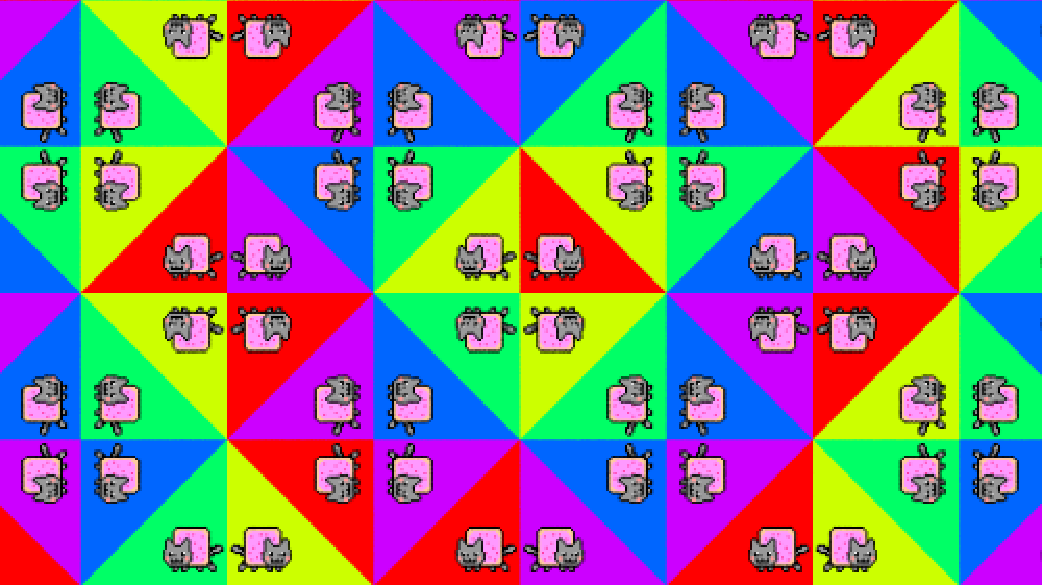
\includegraphics[width=3in, height=3in, keepaspectratio]{../img/tessellation/rightTriangular.pdf}
  \caption{Right triangular tiling}
  \label{fig:rightTriangular}
 \end{minipage}
 \begin{minipage}{0.49\hsize}
  \center
  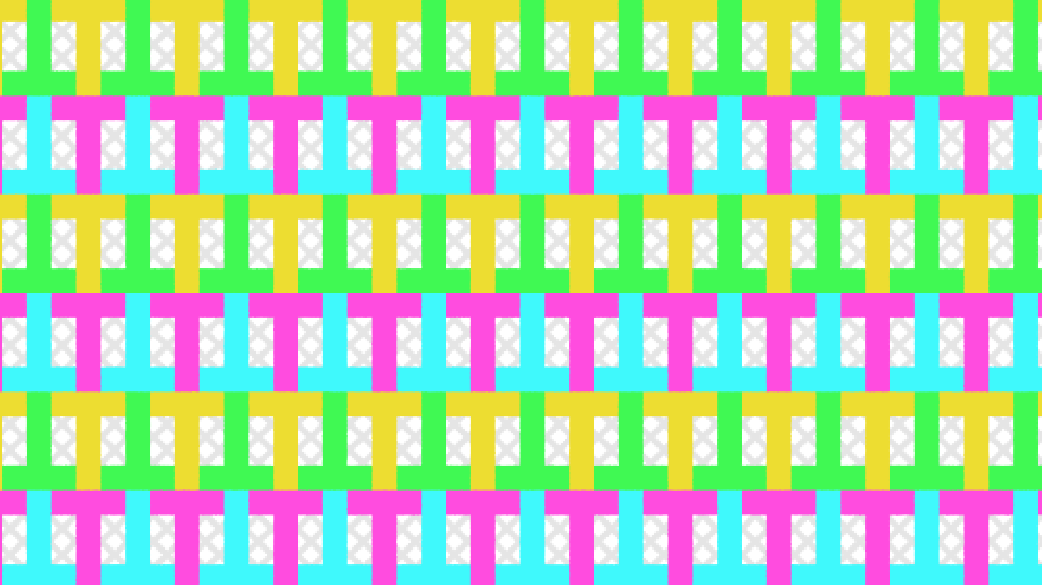
\includegraphics[width=3in, height=3in, keepaspectratio]{../img/tessellation/tessellationT.pdf}
  \caption{Tessellation of alphabet T}
  \label{fig:tessellationT}
 \end{minipage}
\end{figure}

\subsection{About Rendering}

図\ref{fig:rectTile}のような正方形のテセレーションを描画することを考える.
基本的には図\ref{fig:tile}に矢印で示されるような,縦横全4種類の変換の
組み合わせで基本となる正方形を動かすことで, 平面全体を正方形で埋め尽くすことができる.
これは前章でみた群の軌道の描画方法と同様に, 変換の木構造を幅優先探索し,
得られた合成変換で正方形を移動させることで描画することができる.

一方で, シェーダを用いて描画する場合にはその逆を行う.
すなわち,図\ref{fig:tileMove}のように各ピクセルを敷き詰めを構成する4種
の変換で基本タイルへと点を動かす.
そうして,基本タイルへ動かした後で操作の回数や基本タイル上の色からそのピ
クセルの色を決めて塗る.
このアルゴリズムをまとめると以下のような手順になる.
\begin{enumerate}
 \item 基本タイルを見つける
 \item 基本タイルを敷き詰めるための変換を見つける
 \item 各ピクセルを基本タイルに入るまで変換し続ける
 \item 変換の回数や基本タイル上の色を使って色を付ける
\end{enumerate}

\begin{figure}[h!tbp]
   \begin{subfigure}{0.3\textwidth}
   \begin{center}
    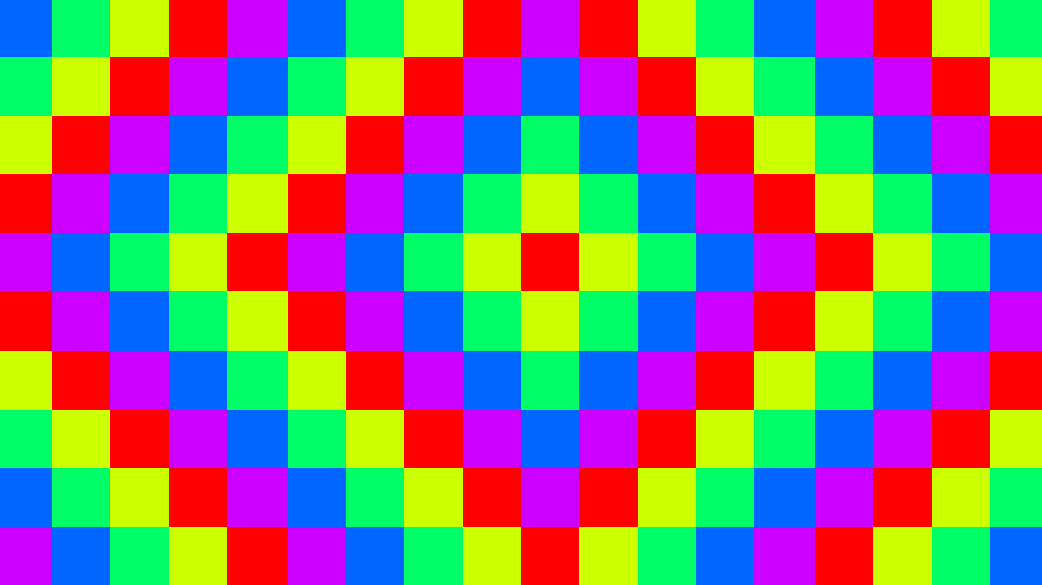
\includegraphics[width=2in, height=2in, keepaspectratio]{../img/tessellation/rectTile.pdf}
    \caption{Rectangular tiling}
    \label{fig:rectTile}
   \end{center}
  \end{subfigure}
 \hspace*{\fill}
   \begin{subfigure}{0.3\textwidth}
   \begin{center}
    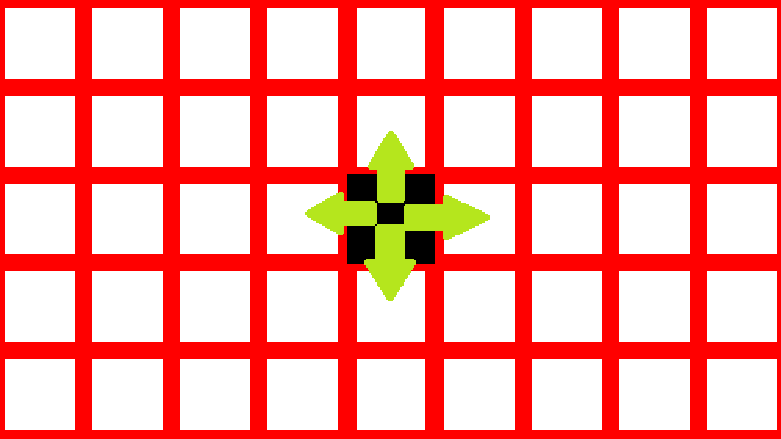
\includegraphics[width=2in, height=2in, keepaspectratio]{../img/tessellation/tile.pdf}
    \caption{Tile and transformations}
    \label{fig:tile}
   \end{center}
  \end{subfigure}
 \hspace*{\fill}
 \begin{subfigure}{0.3\textwidth}
  \begin{center}
   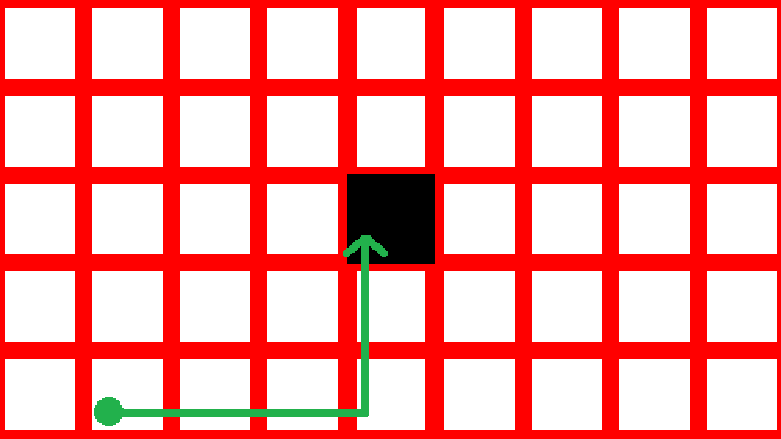
\includegraphics[width=2in, height=2in, keepaspectratio]{../img/tessellation/tileMove.pdf}
   \caption{Move}
   \label{fig:tileMove}
  \end{center}
 \end{subfigure}
 \hspace*{\fill}
\caption{Tile}
\end{figure}

ユークリッド平面上での敷き詰め模様は,数学的に分類がされている.
この分類に関しては『装飾パターンの法則』
\cite{tessellationDesign}が詳しい.
この本では主にデザイナーに向けて, 装飾に用いられる敷き詰め模様の法則性,
分類について記述されており, 敷き詰め模様のデザインへの応用に役立つ.

より数学的にまとめられた文献にはMartin von Gagern, Jrgen
Richter-Gebertによる\cite{hyperbolization}がある.
この論文はユークリッド平面上での敷き詰め模様を双曲平面での敷き詰めに変換
する方法を提案したものであるが, 敷き詰め模様の分類についても詳しい.
また,Martin von Gagernによる\emph{morenaments}\footnote{morenaments:
\url{http://www.morenaments.de/}}というソフトウェアを用いることで, 各敷
き詰めパターンの挙動をみることができる.

\subsection{Hyperbolic Tessellation}

我々が普段見ている世界を考えるユークリッド幾何学では, 平面上に任意の直線
$L$とその直線上にない点$P$がある時, $P$を通り, $L$に平行な直線は一本しか
引くことができない.
これは平行線公準とよばれている.
ボヤイ, ロバチェフスキー, ガウスといった数学者はそれぞれ
こういった公理を崩した幾何学のモデルの一つである\emph{双曲幾何
学}(\textit{Hyperbolic Geometry})を考案した.
双曲幾何学では, $L$に平行な直線を無限に引くことができる.
また, 最も特徴的なのは三角形の内角の和が180度以下になるということである.

双曲幾何学における平面, 双曲平面における敷き詰め模様が\emph{双曲テセレー
ション}{\it (Hyperbolic Tessellation)}とよばれる.
双曲幾何学のモデルとして有名なものに\emph{ポアンカレの円盤モデ
ル}(\textit{Poincar\'e disk model})や\emph{ポアンカレの上半平面モデ
ル}(\textit{Poincar\'e half-plane model})がある.
図\ref{fig:hyperbolicTessellation}に円盤モデル, 図\ref{fig:upperHalf}に
上半平面モデルとこれらのモデルにおけるテセレーションを示した.
画家のM.C.エッシャーはこのような図に影響されて『天使と悪魔』や『Circle
Limit』といった有名な作品を生み出した.

円盤モデルにおいては図\ref{fig:hyperbolicTessellation}に示される円盤が双
曲平面であり, 世界のすべてである.
円盤の端がユークリッド平面における無限遠点となる.
また, 双曲平面では円弧が直線となり, あらゆるタイルが円弧で構成される.

\begin{figure}[h!tbp]
 \begin{minipage}{0.49\hsize}
  \center
  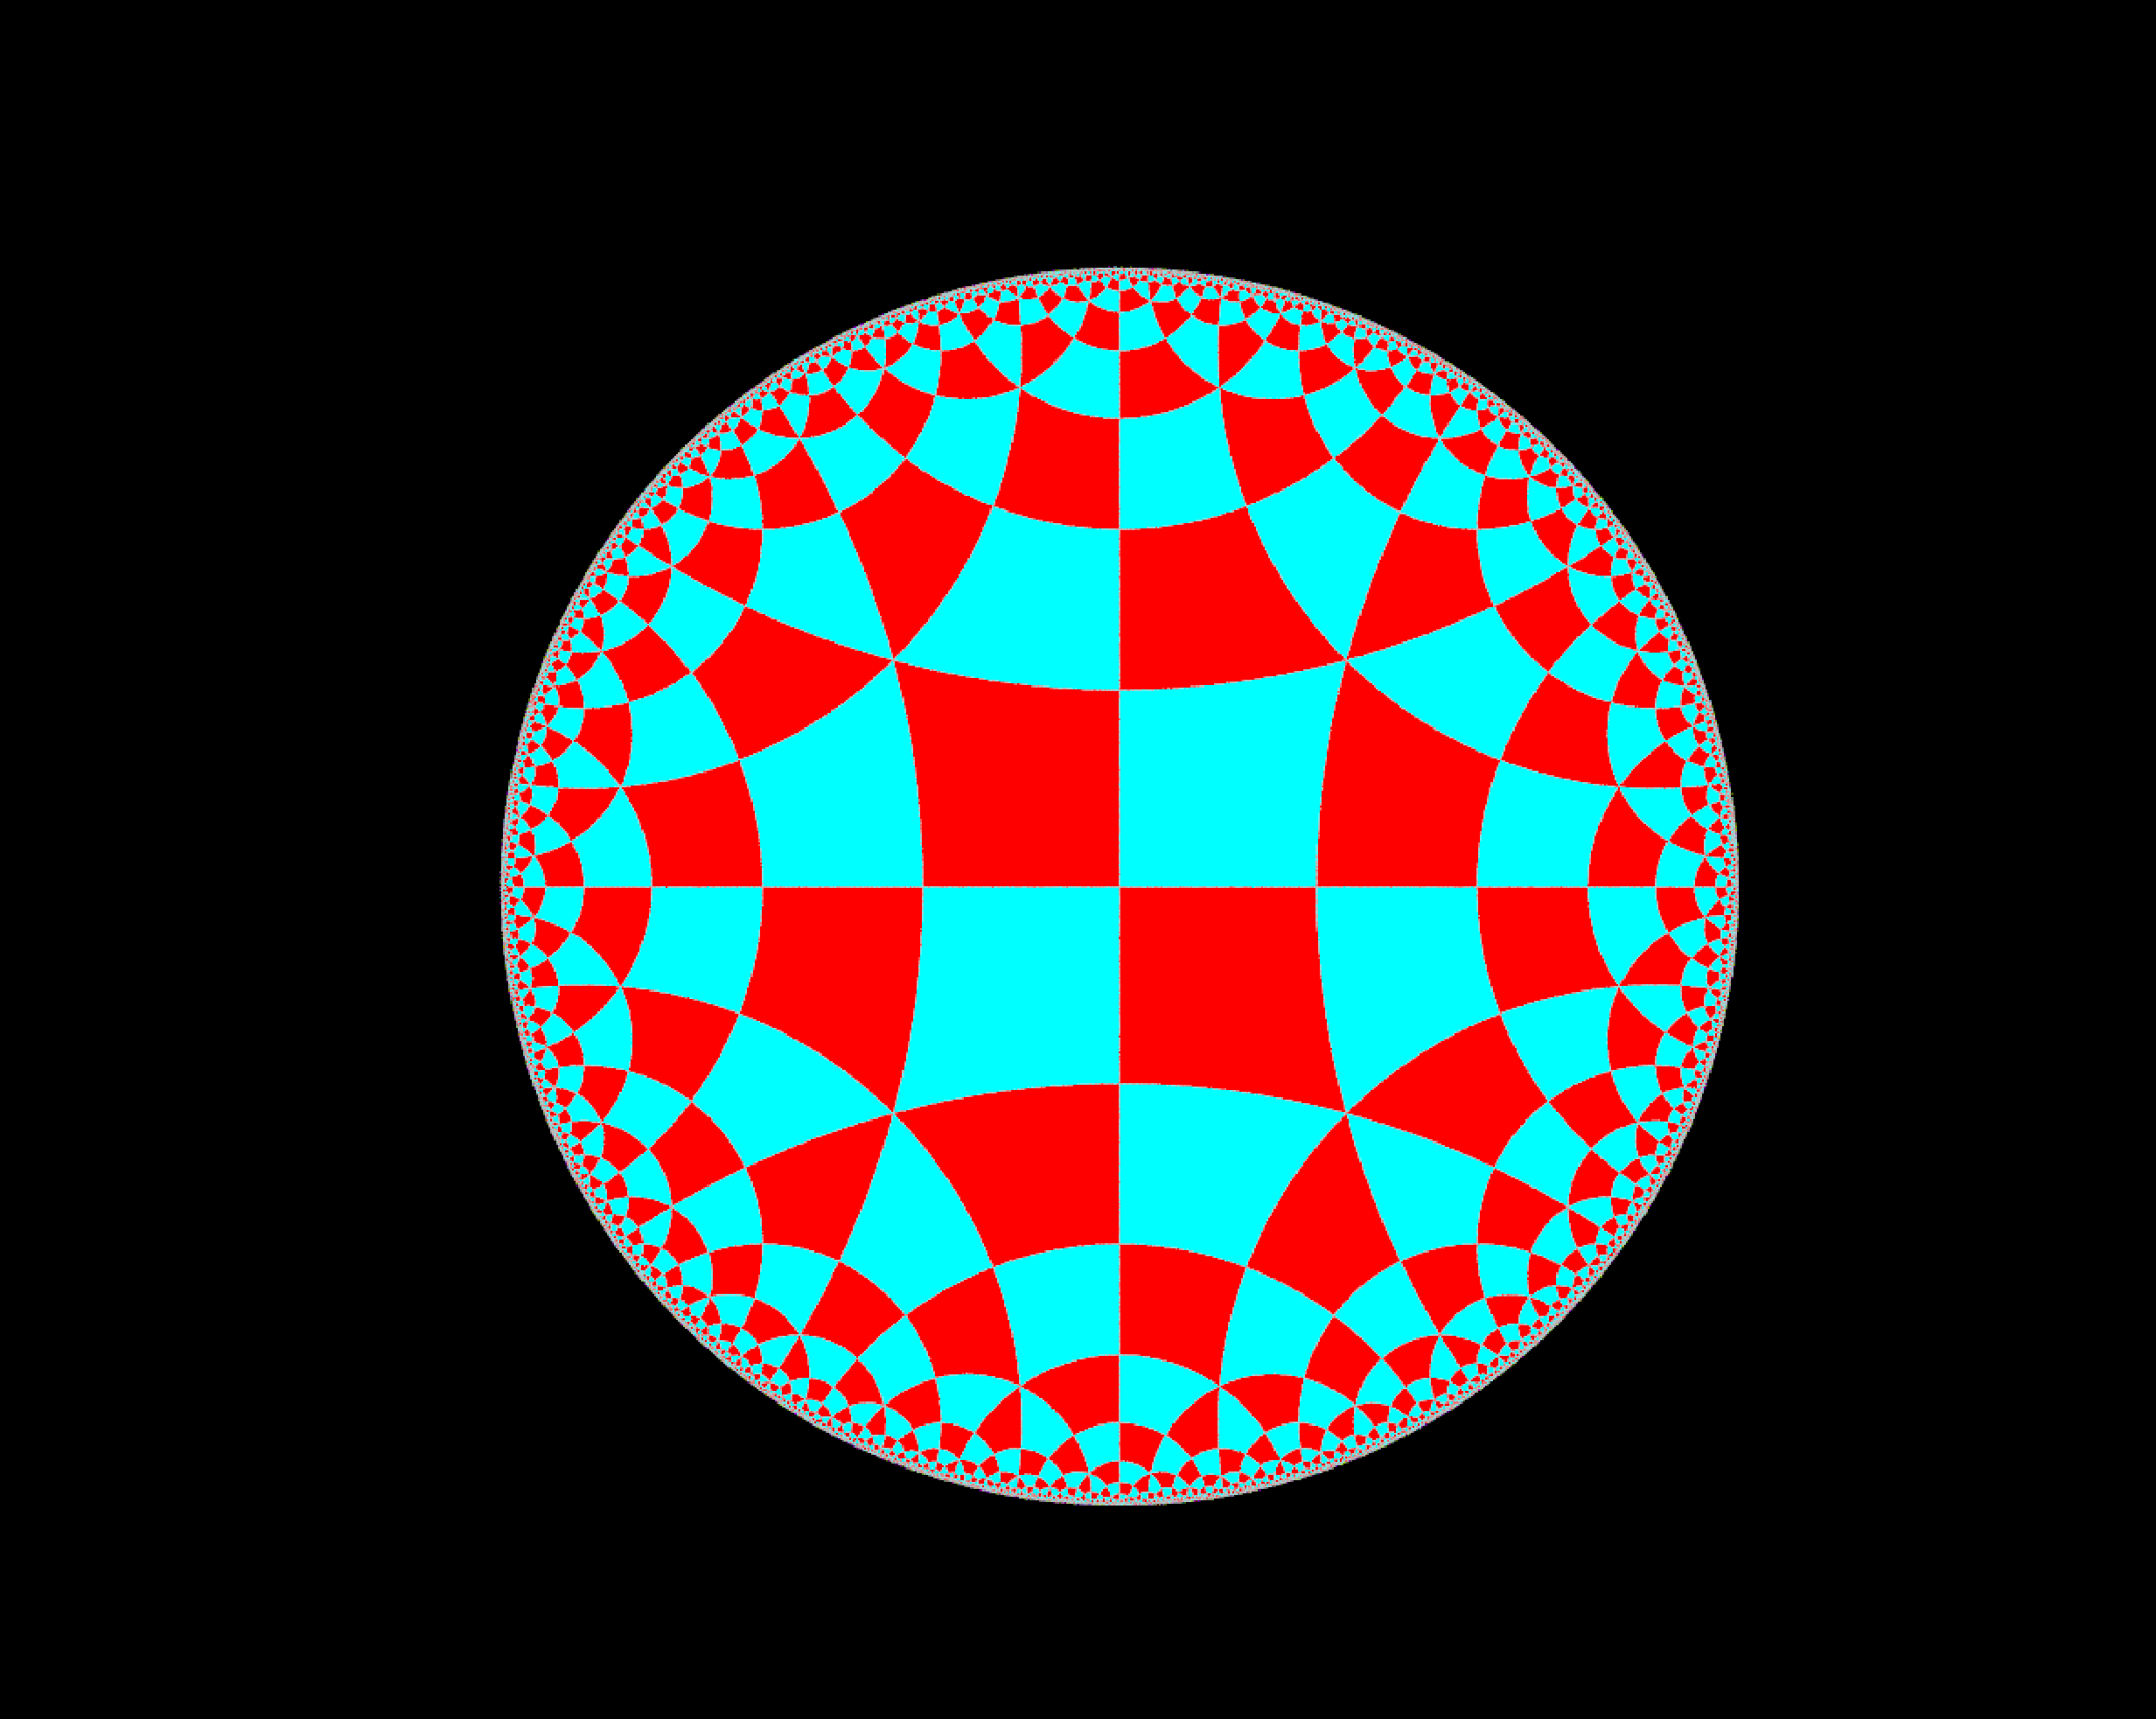
\includegraphics[width=3in, height=3in,
  keepaspectratio]{../img/tessellation/hyperbolicTessellation.pdf}
  \caption{Hyperbolic Tessellation}
  \label{fig:hyperbolicTessellation}
 \end{minipage}
 \hspace*{\fill}
 \begin{minipage}{0.49\hsize}
  \center
  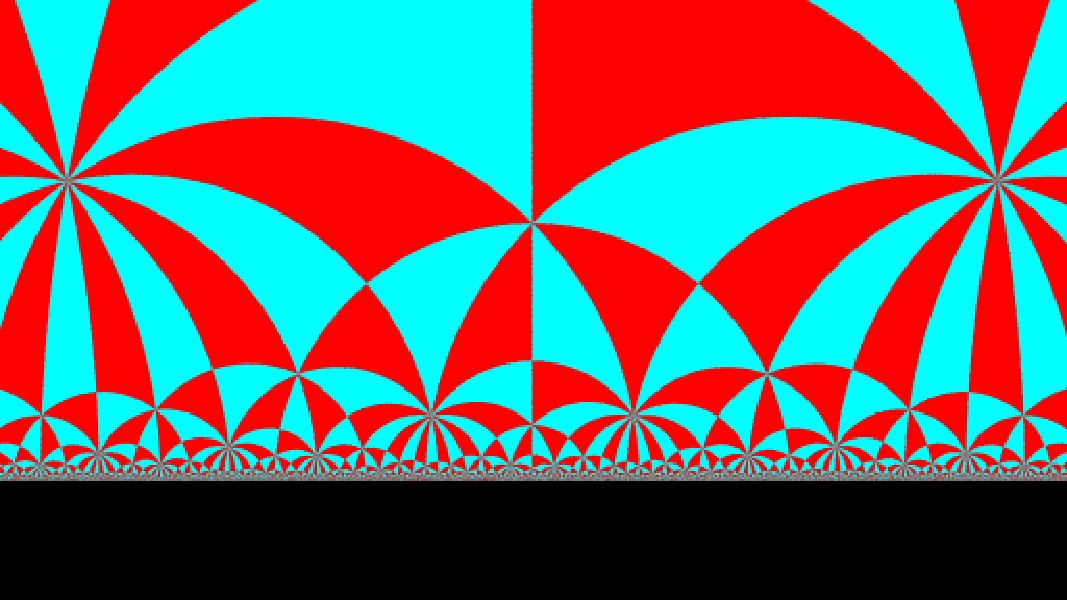
\includegraphics[width=3in, height=3in, keepaspectratio]{../img/tessellation/upperHalf.pdf}
  \caption{Upper half model}
  \label{fig:upperHalf}
 \end{minipage}
\end{figure}

これより円盤モデルにおけるテセレーションを描く方法を記述する.
円盤モデルの円盤は原点中心,半径1の円とする.
基本タイルを中央にある4つの最も大きなタイルの内の1つとする.
このタイルはx軸,y軸,そして2つの円弧で囲まれている.
これらの弧に関する反転を用いて,先ほどのアルゴリズムを用いると図
\ref{fig:hyperbolicTessellation}のような敷き詰め模様を描くことができる.
円盤の内側に属する点は内側の基本タイルに,円盤の外側に属する点は外側の基
本タイルに移るため,最終的な点の位置で処理を切り分けることにより,両者の
色を区別することができる.
双曲タイリングは,木構造の探索によって計算しようとすると,計算量が多くな
るため,円盤の端まで描画することは難しいが,前述のアルゴリズムを用いると
端までリアルタイムで描画することができる.

図\ref{fig:outer}では基本タイルとして,3つの角が$\frac{\pi}{2}$,残りの角が$\frac{\pi}{3}$である4辺形を用いたが,基本タイルでも敷き詰めることができるわけではない.
敷き詰め条件は\emph{ポアンカレの張り合わせ定理}として知られている.双曲三角形のタイリング条件は以下のようになる.
\begin{eqnarray*}
\text{3内角を}\frac{\pi}{p},\frac{\pi}{q},\frac{\pi}{r}\text{とする時,}
 \frac{1}{p} + \frac{1}{q} + \frac{1}{r} < 1 \text{を満たす.}
\end{eqnarray*}
双曲三角形を2つ張り合わせることで双曲4辺形を得ることができる.

Vladimir Bulatov氏は円盤を変形させる方法を考案した\cite{bending}.Bulatov氏は双曲平面や双曲空間におけるタイリングや,その変形についてまとめている\footnote{Bulatov Abstract Creations: \url{http://bulatov.org/math/index.html}}.
筆者は図\ref{fig:deformed}のような双曲タイリングとその変形を行うWebアプリケーションを制作している.
\footnote{Hyperbolic Tessellator: \url{https://soma-arc.net/HyperbolicTessellator/}}.

\begin{figure}[htbp]
  \begin{minipage}{0.49\hsize}
   \center
   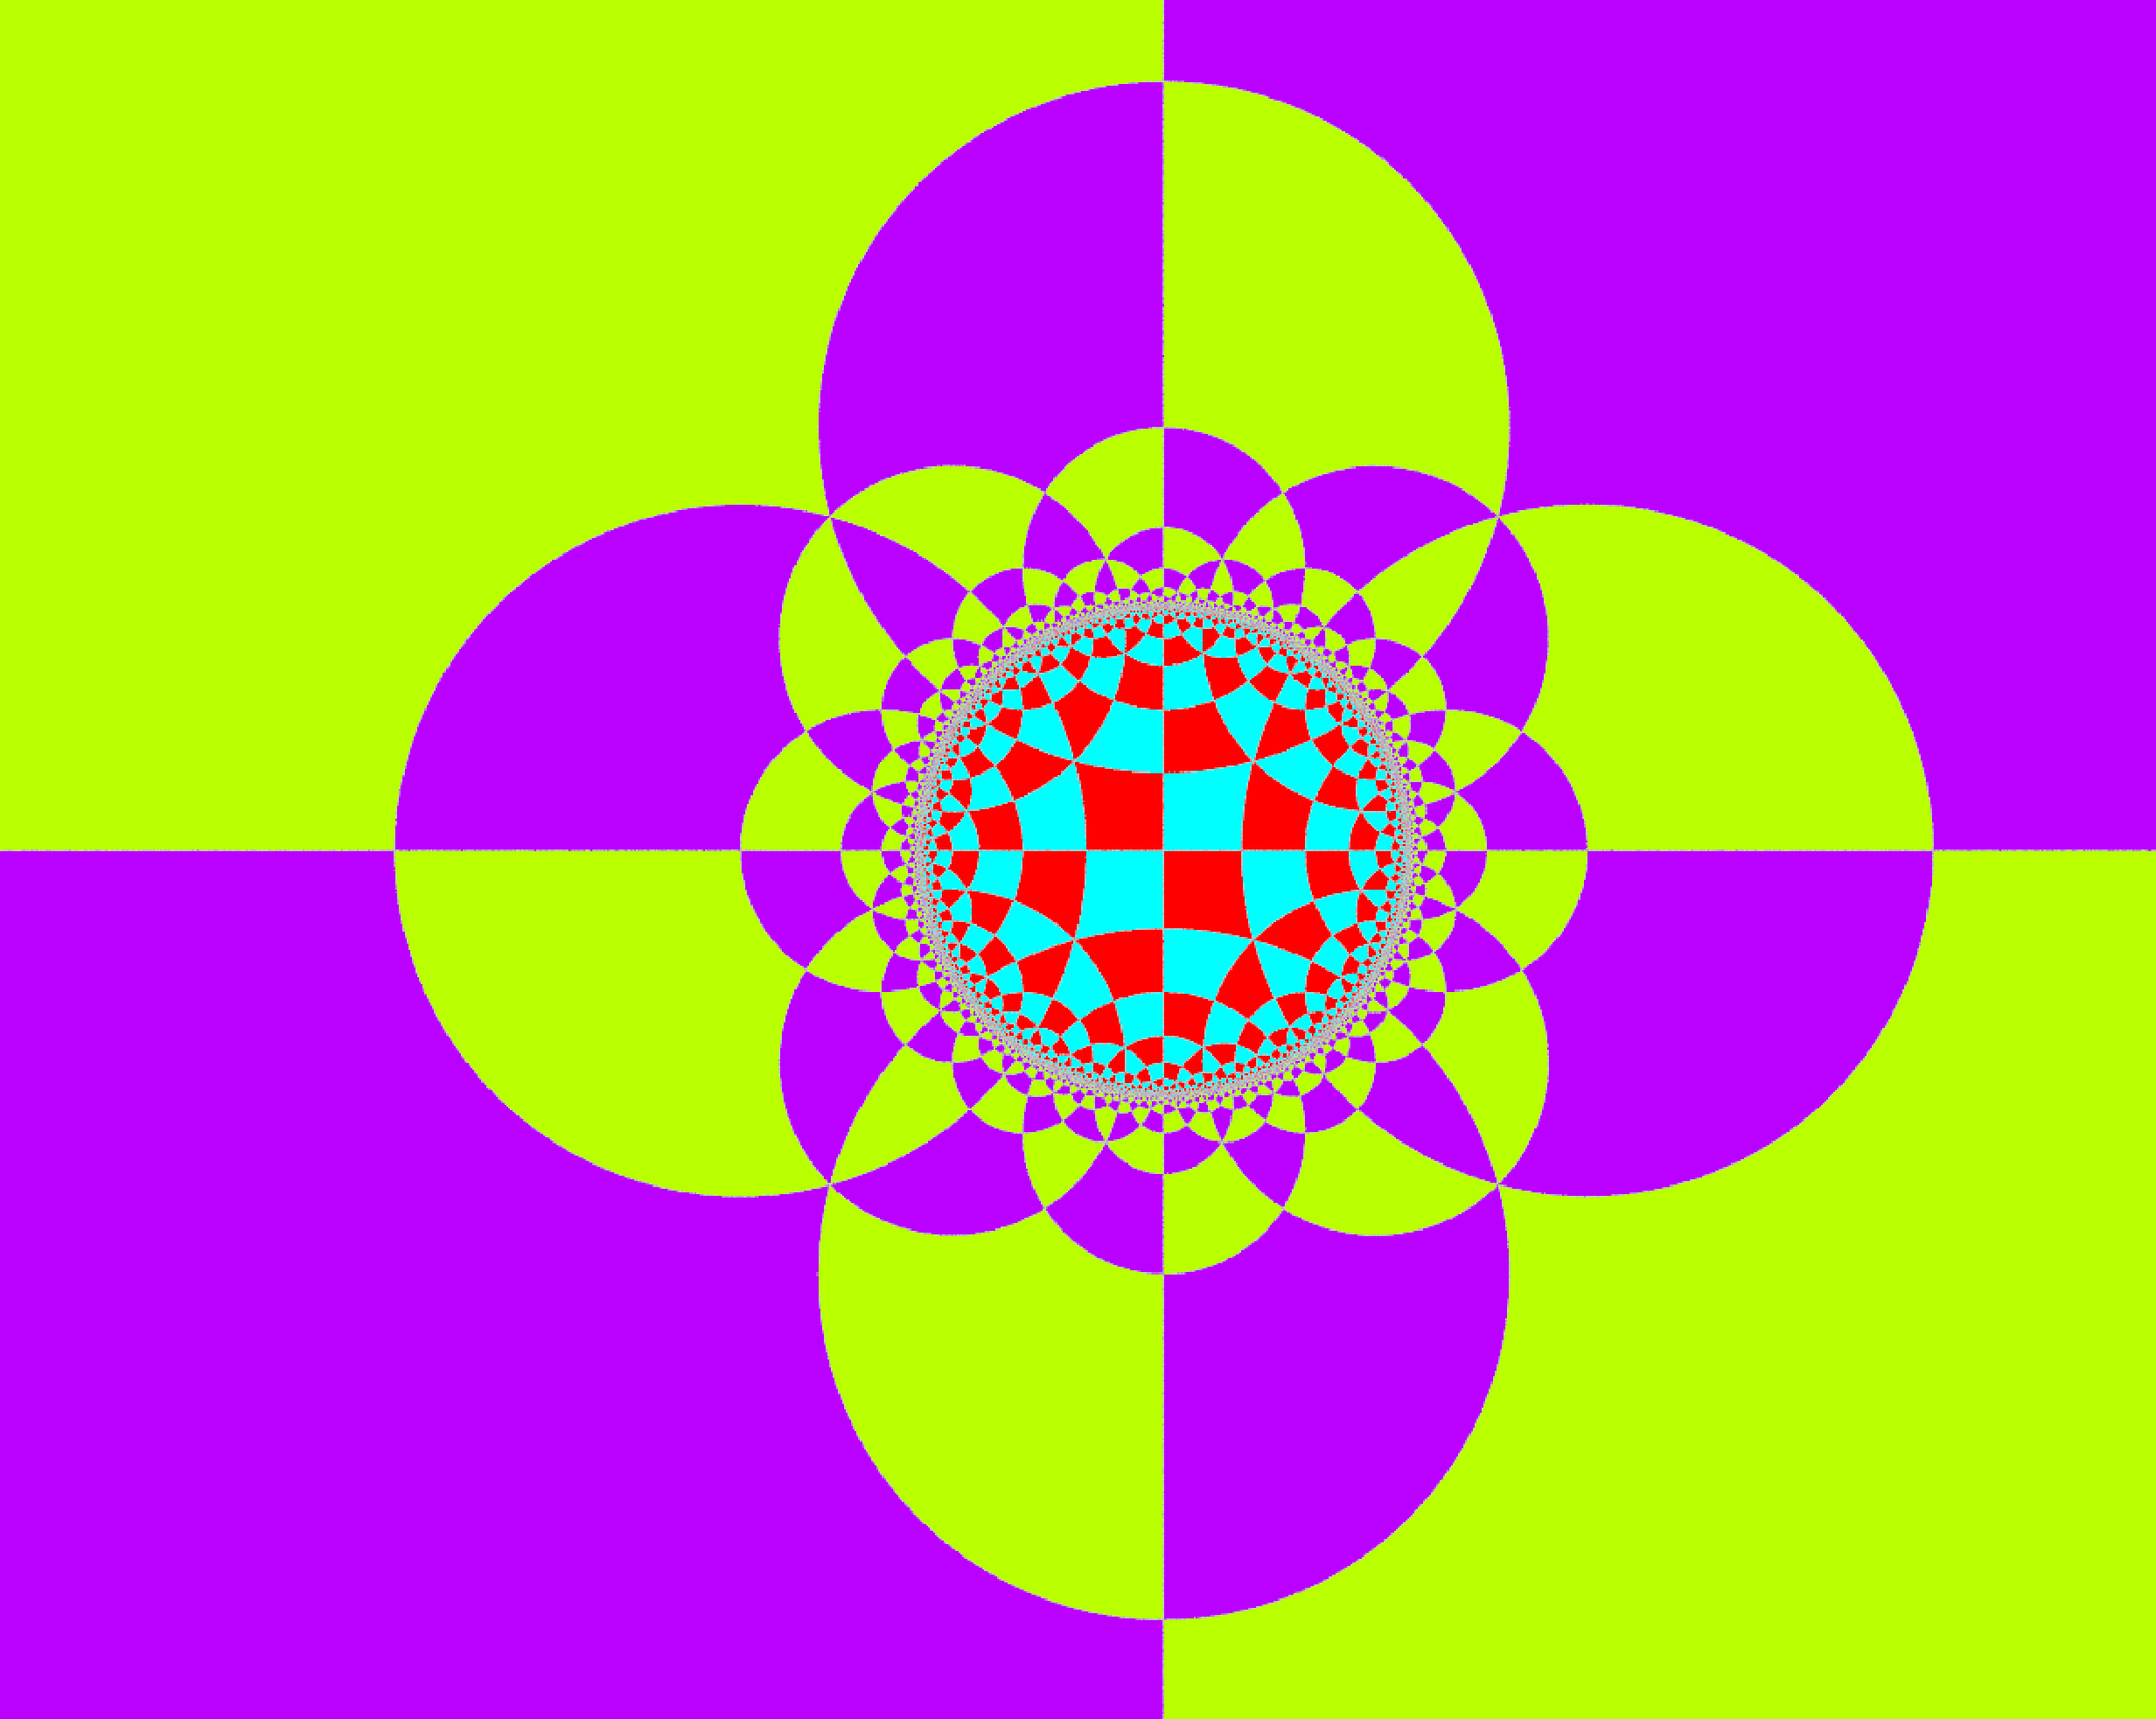
\includegraphics[width=3in, height=3in, keepaspectratio]{../img/tessellation/outer.pdf}
   \caption{Outer}
   \label{fig:Outer}
  \end{minipage}
 \hspace*{\fill}
 \begin{minipage}{0.49\hsize}
  \center
  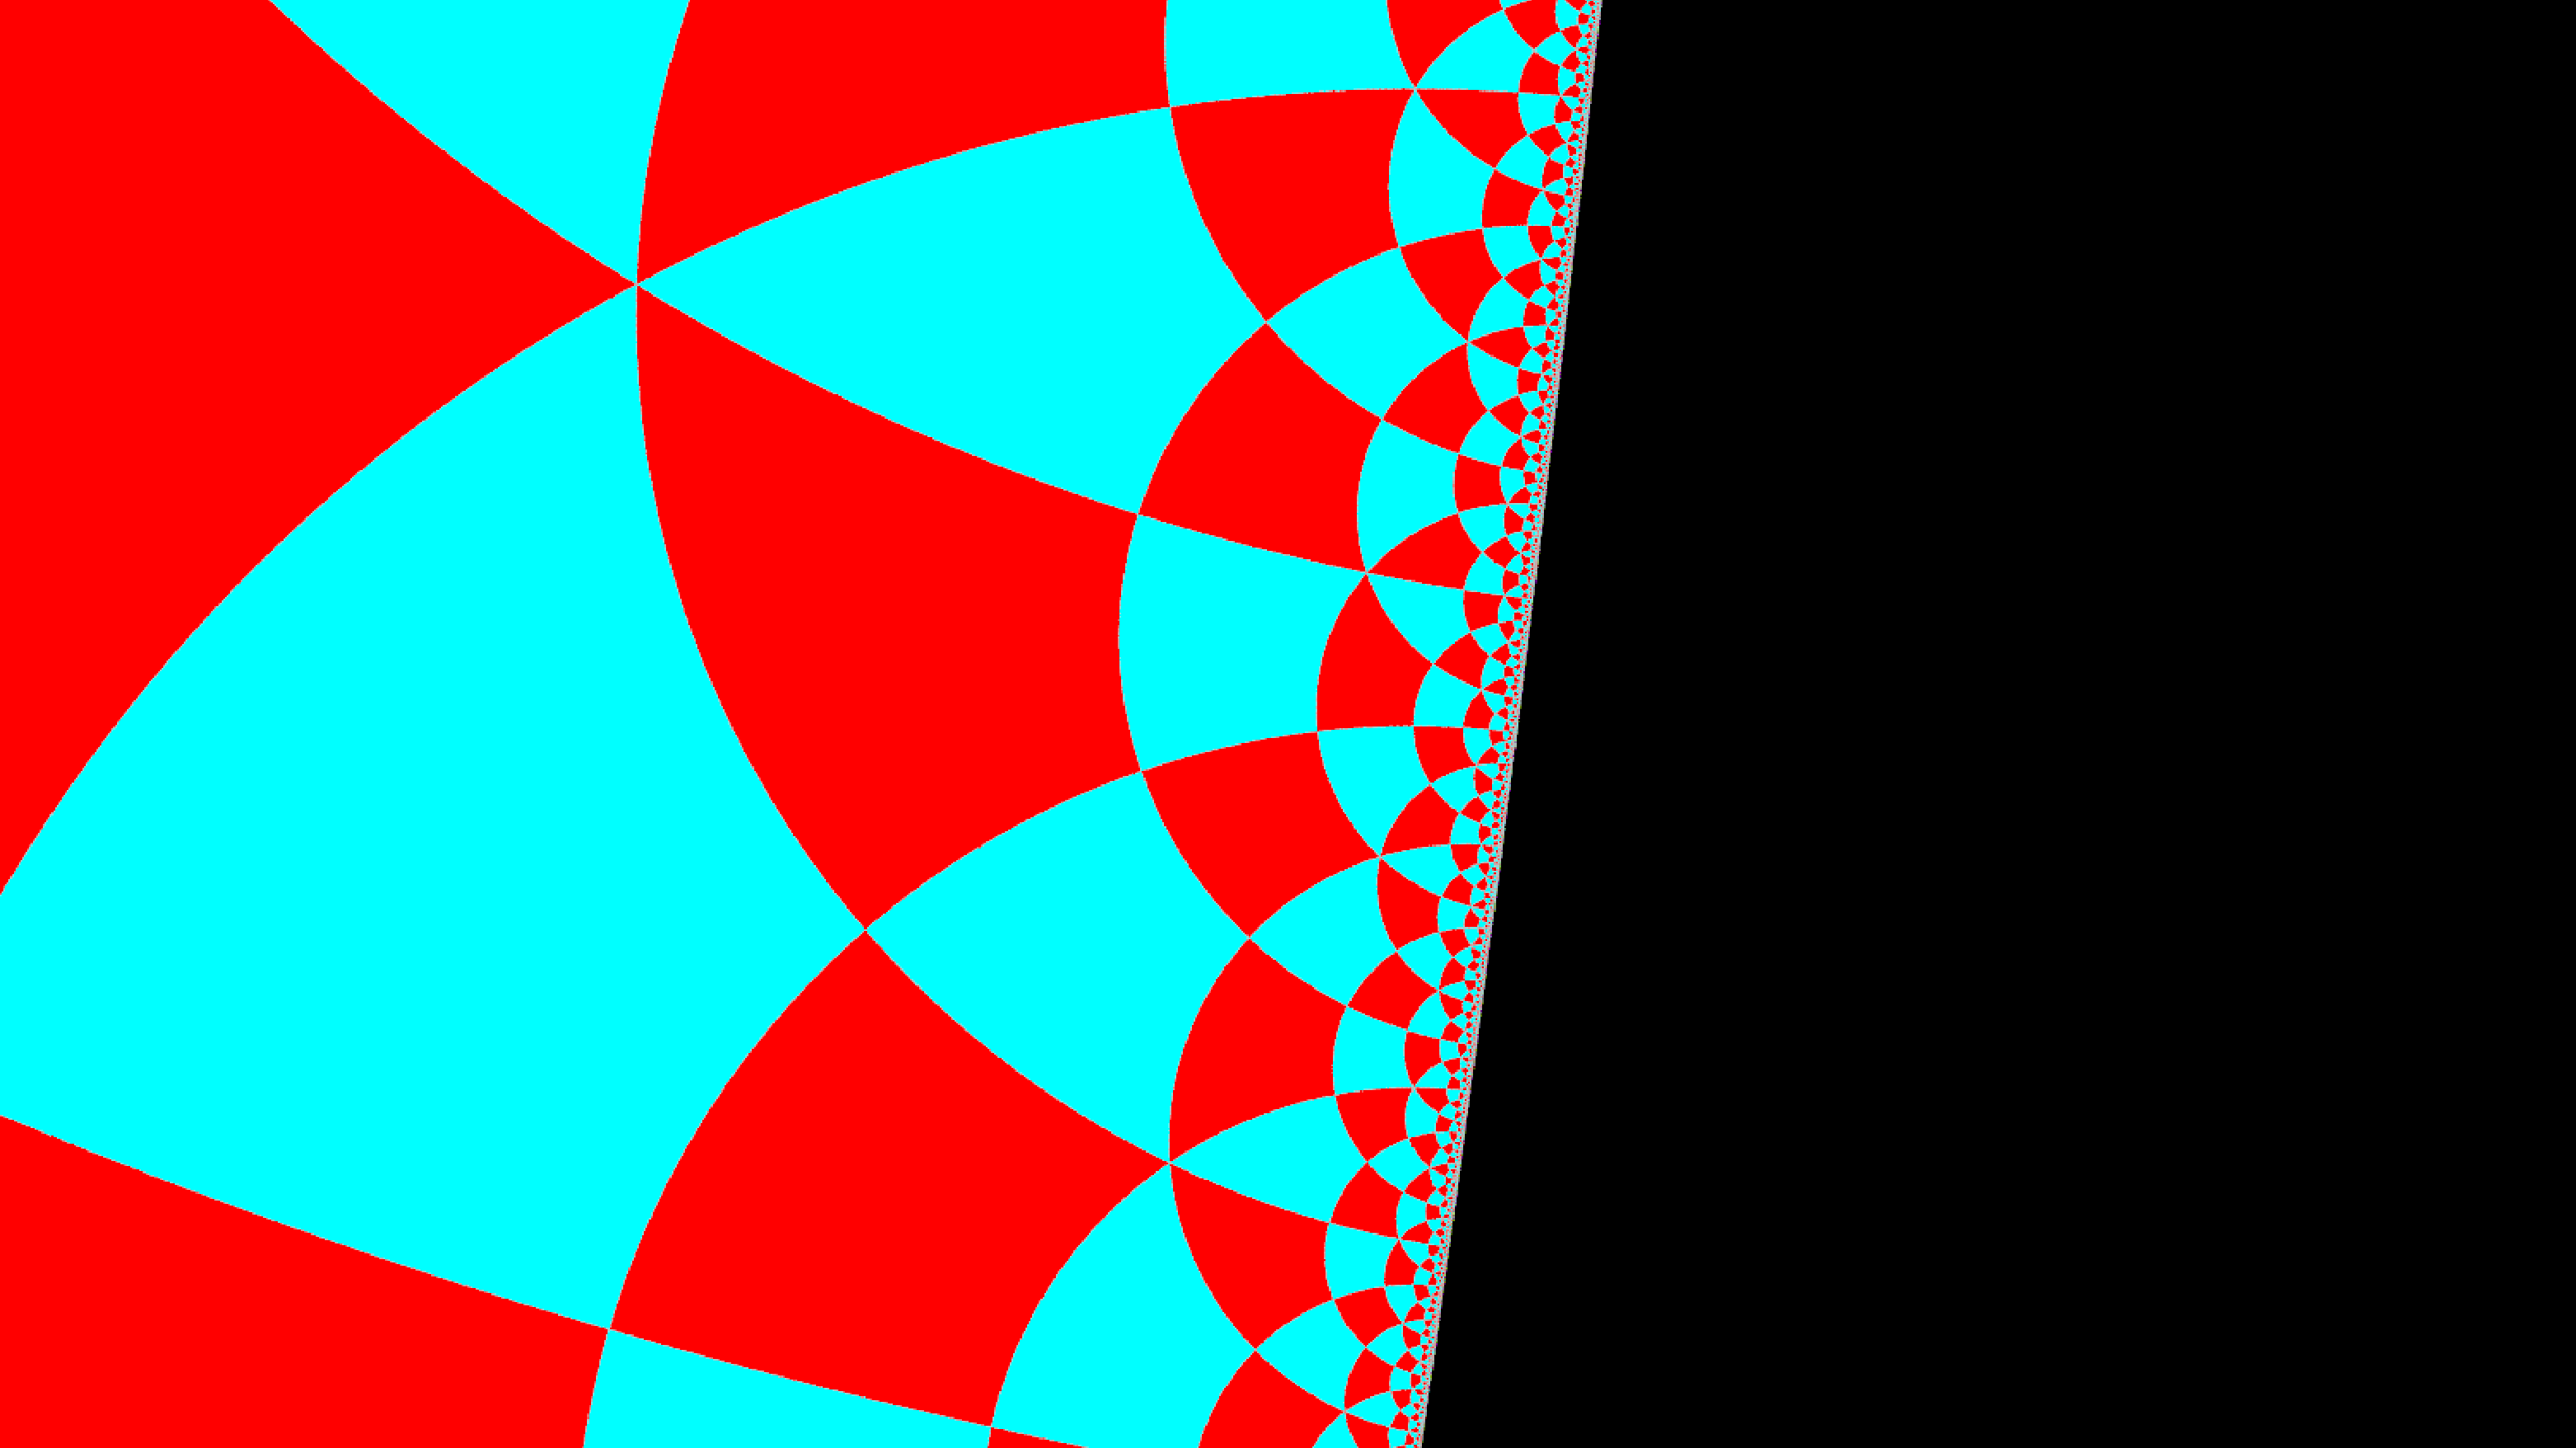
\includegraphics[width=3in, height=3in, keepaspectratio]{../img/tessellation/zoom.pdf}
  \caption{zoom}
  \label{fig:zoom}
 \end{minipage}
\end{figure}


\begin{figure}[htbp]
  \begin{minipage}{0.49\hsize}
   \center
   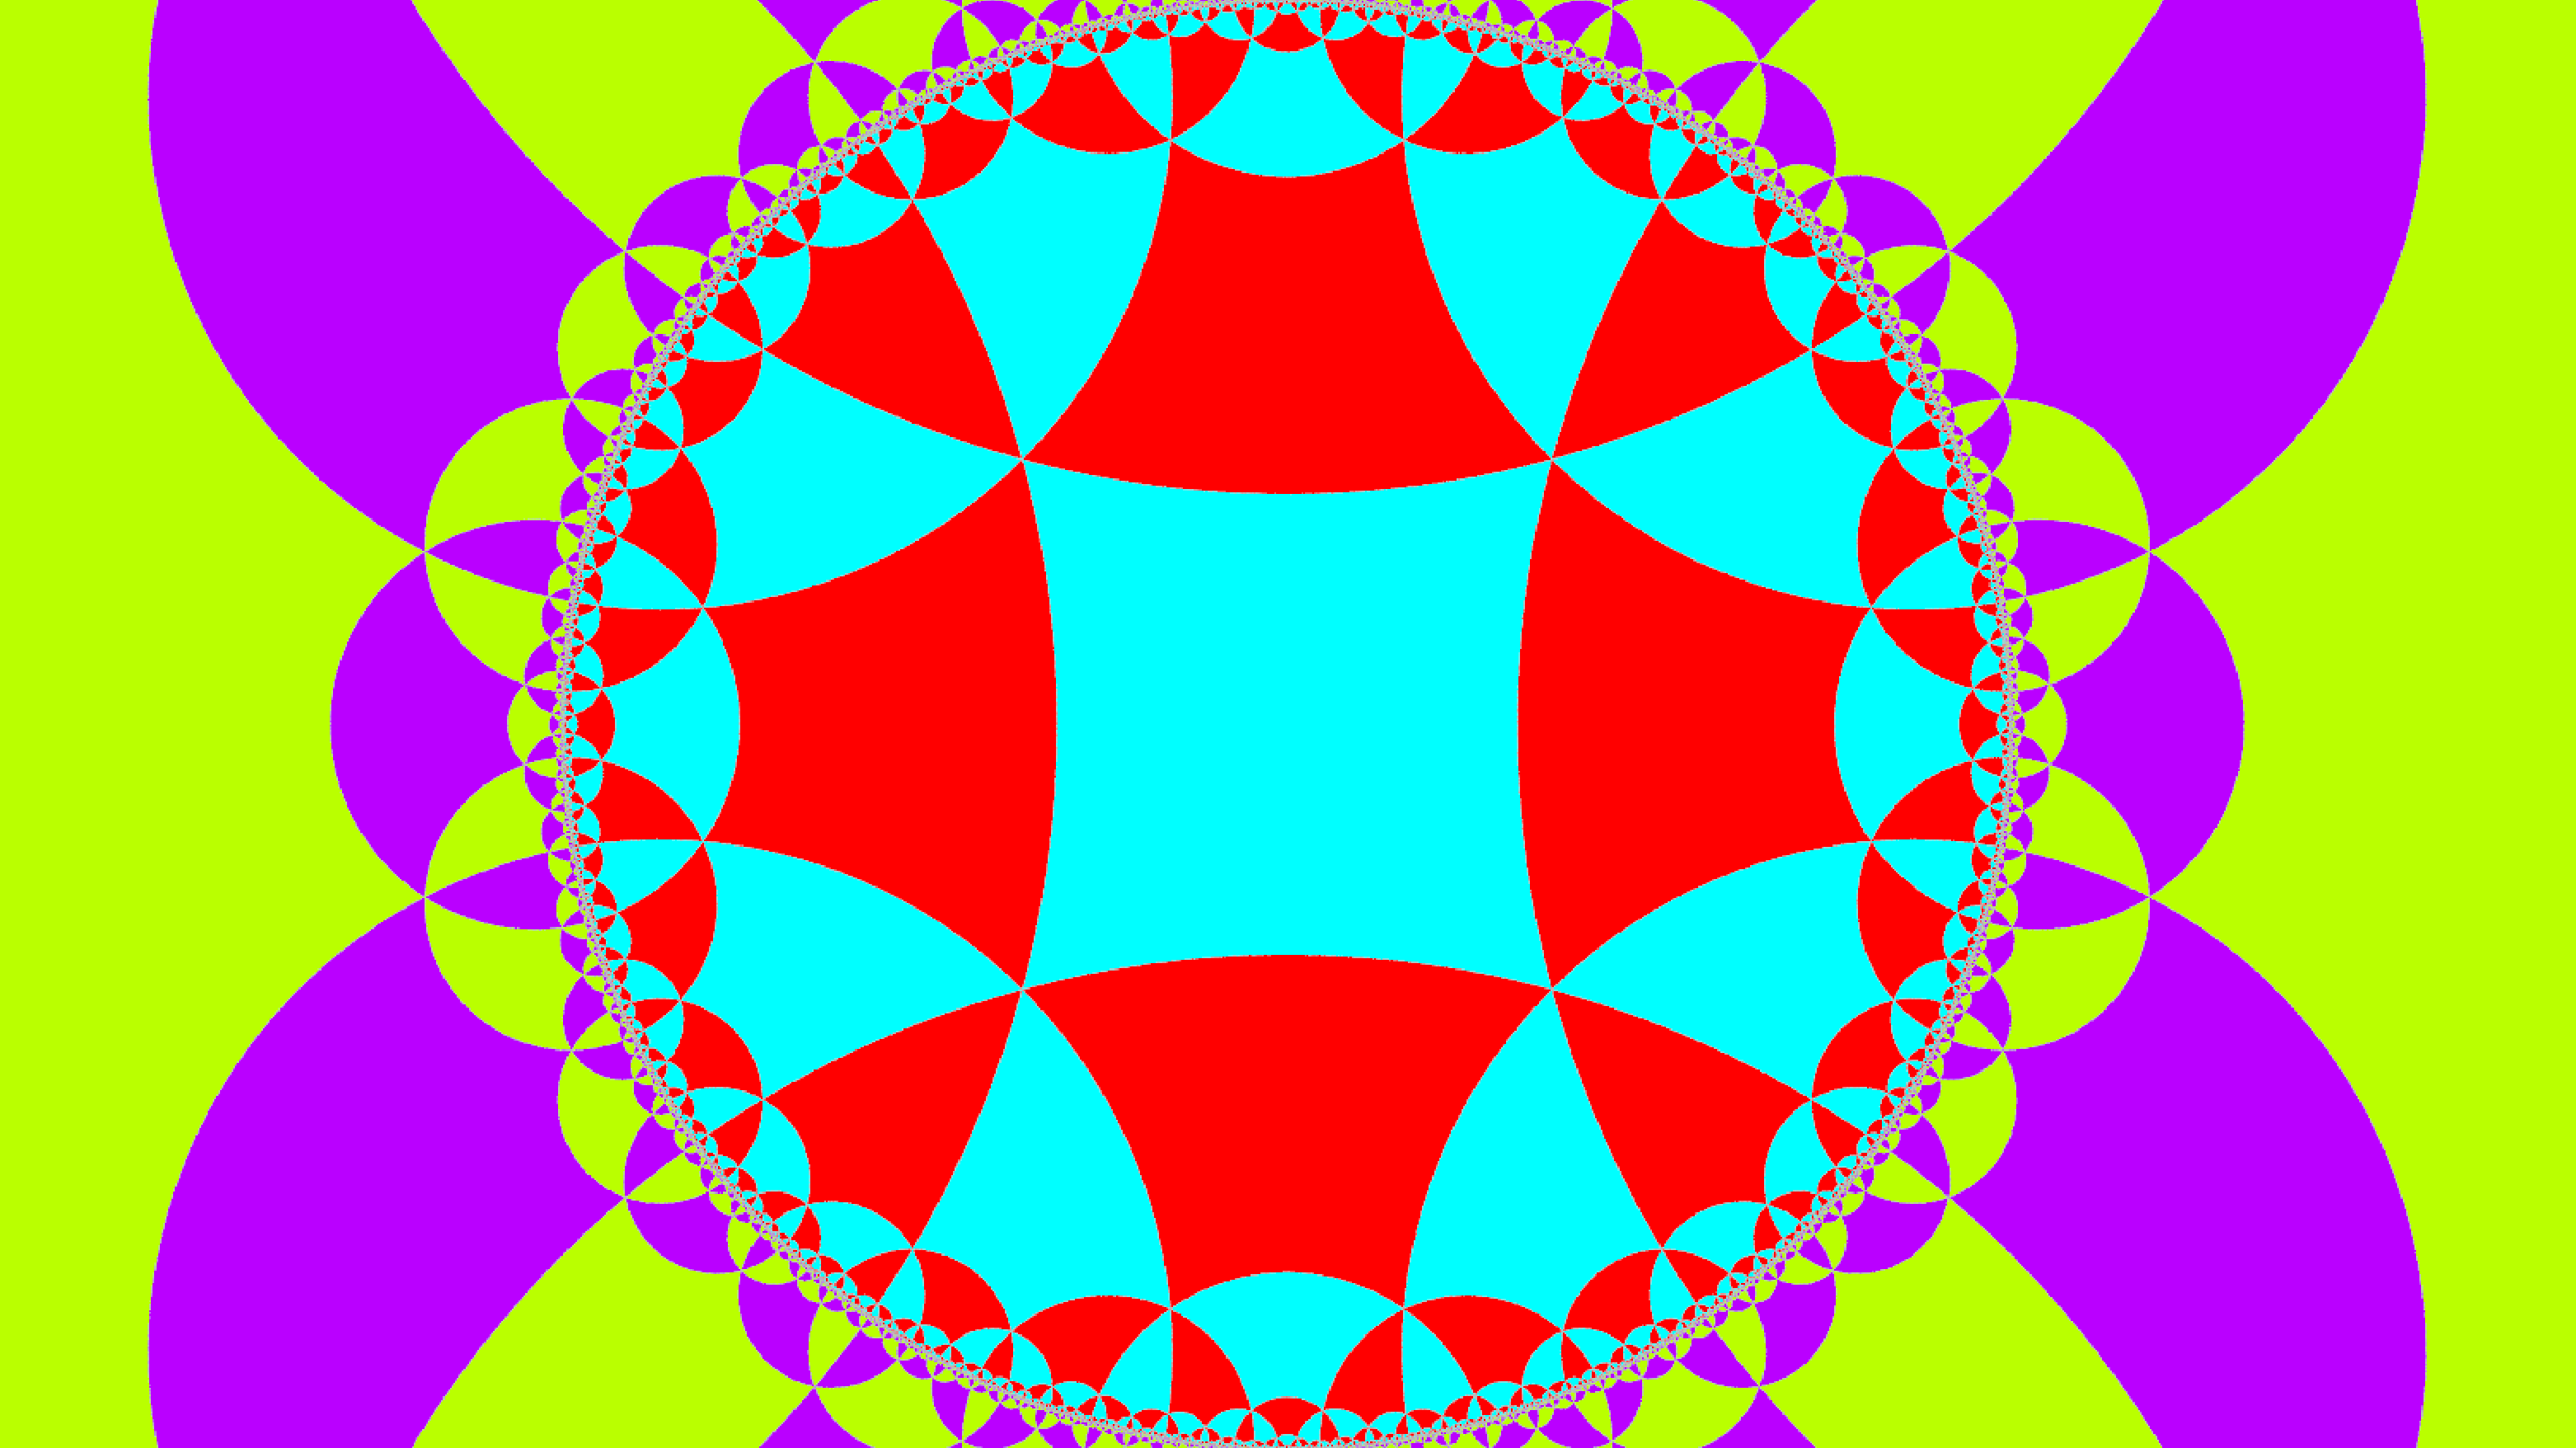
\includegraphics[width=3in, height=3in, keepaspectratio]{../img/tessellation/hyperbolicRect}
   \caption{rect}
   \label{fig:rect}
  \end{minipage}
 \hspace*{\fill}
 \begin{minipage}{0.49\hsize}
  \center
  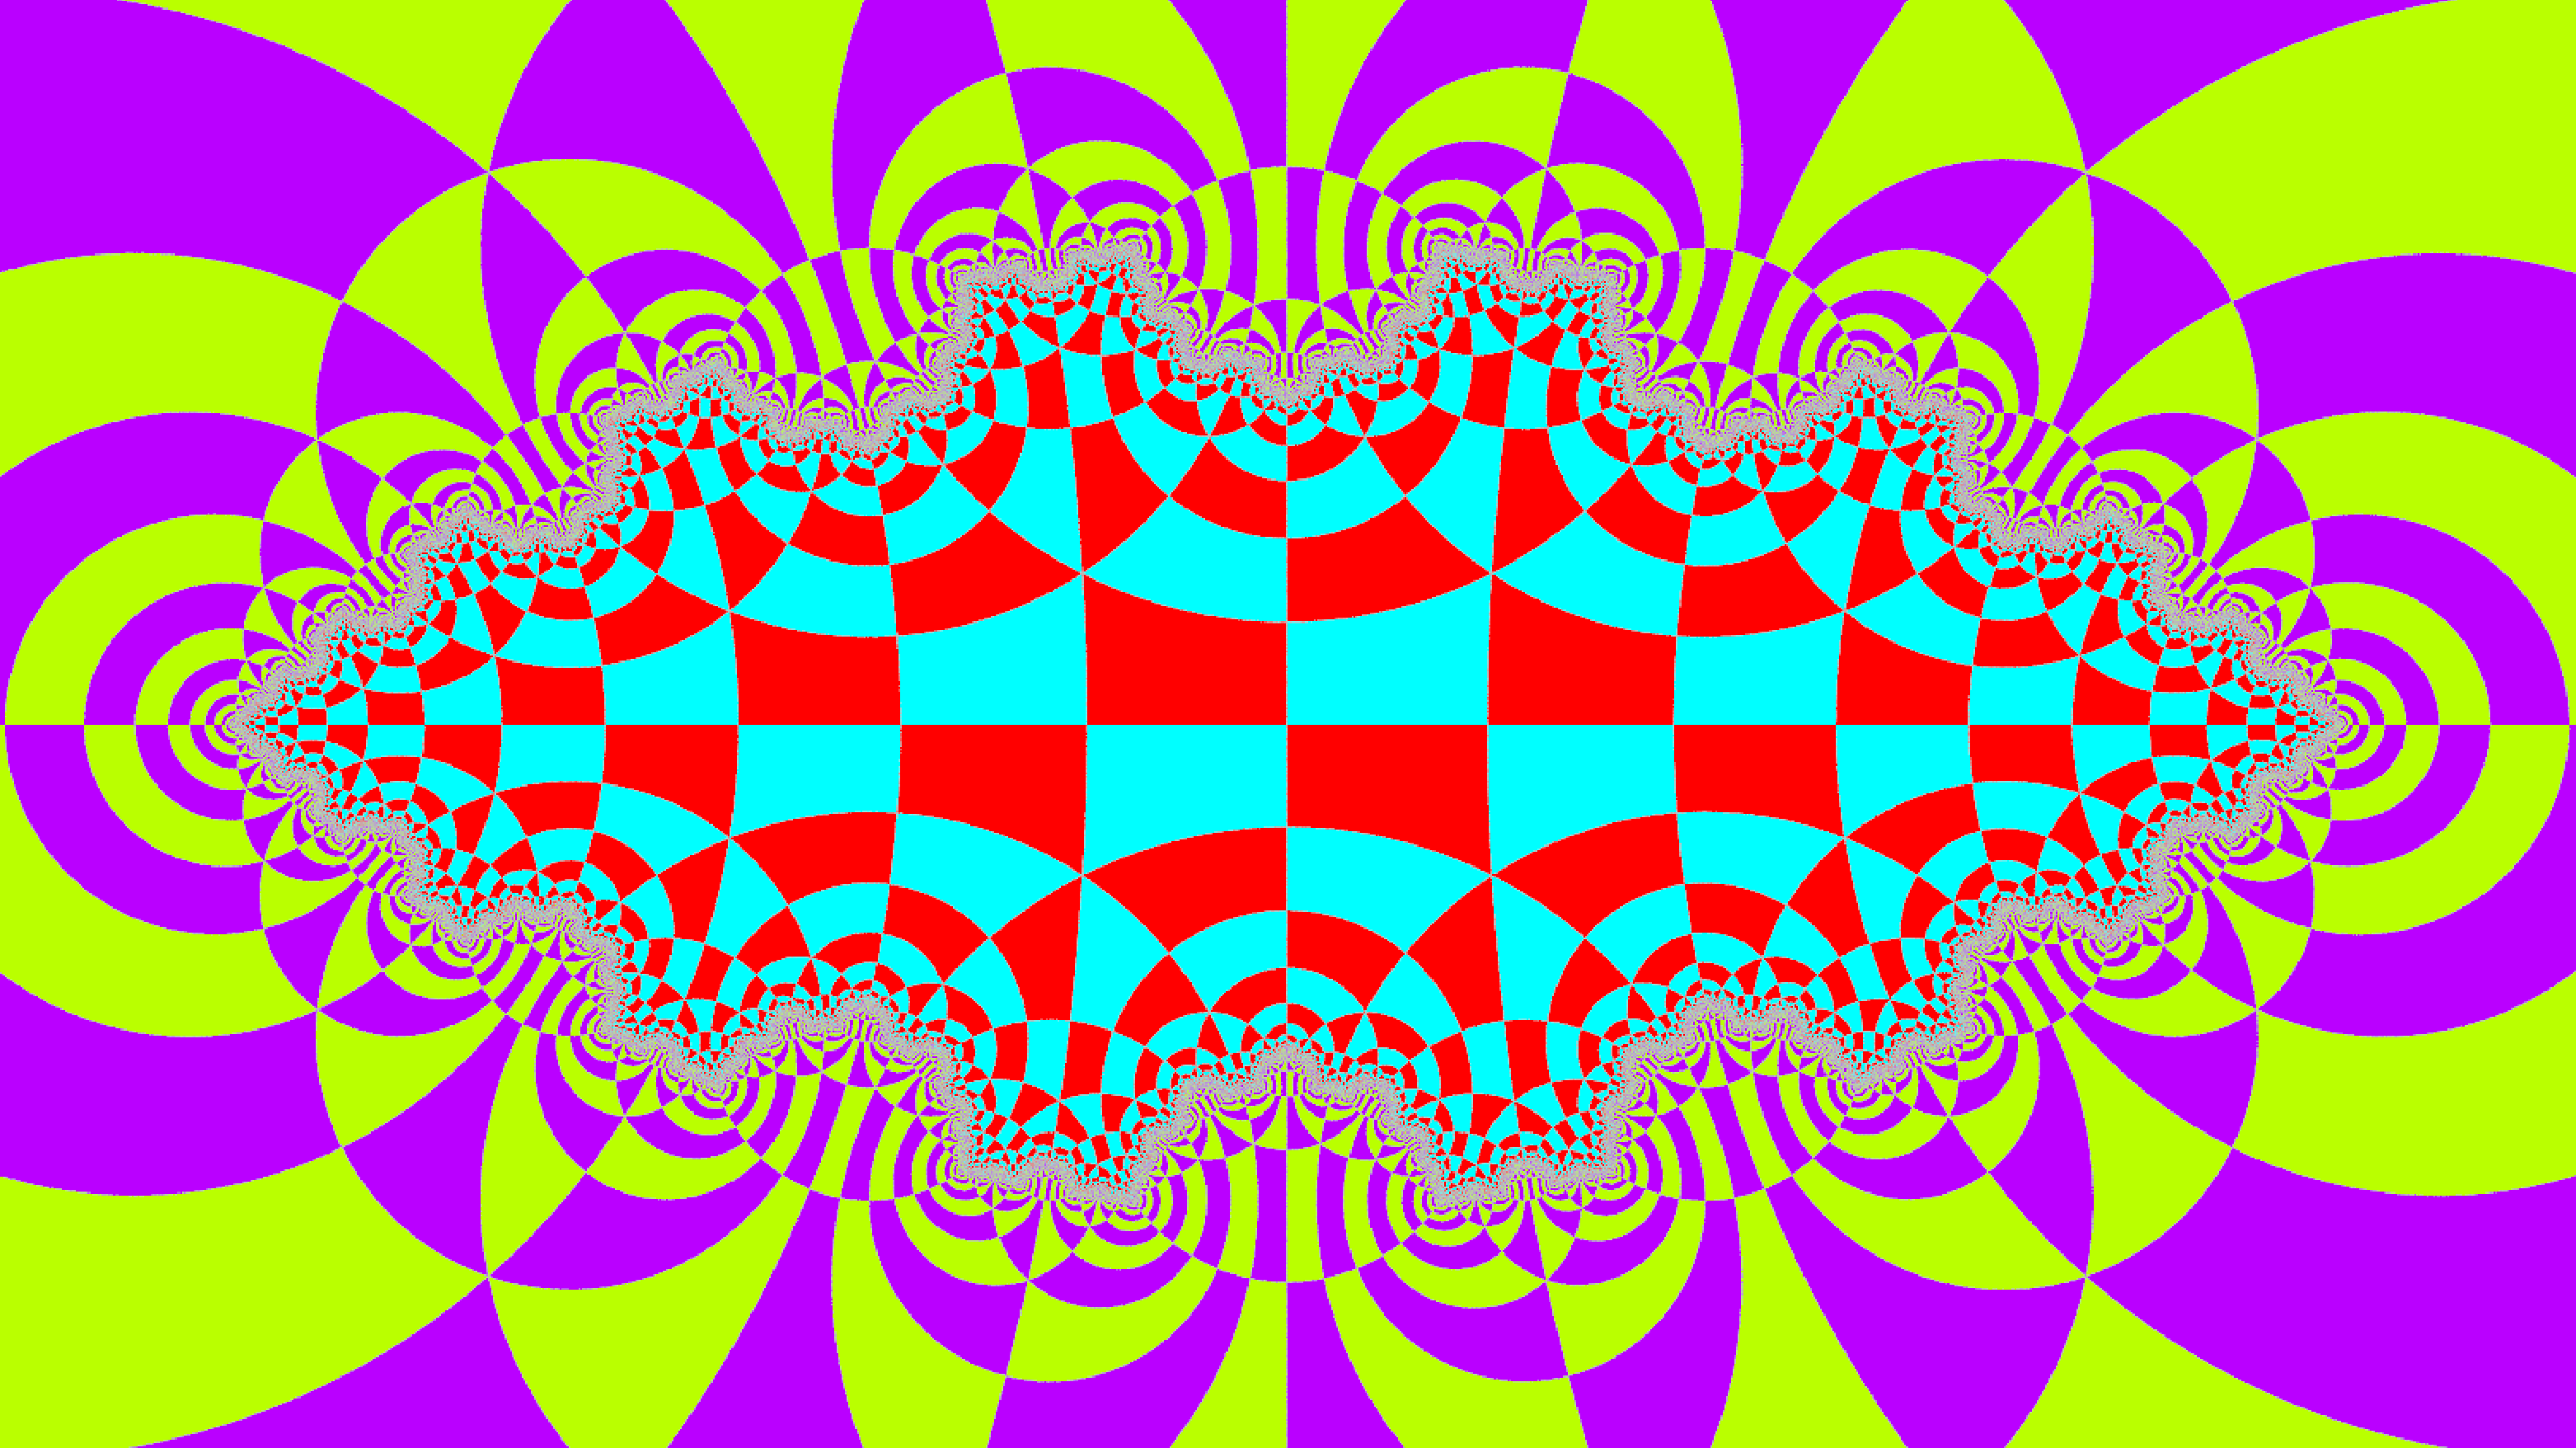
\includegraphics[width=3in, height=3in, keepaspectratio]{../img/tessellation/deformed.pdf}
  \caption{deformed}
  \label{fig:deformed}
 \end{minipage}
\end{figure}

\clearpage